\documentclass[11pt]{article}
\usepackage{fullpage,amsmath,amssymb,amsthm}
\usepackage[title]{appendix}
\usepackage[T1]{fontenc}
\usepackage{lmodern}
\usepackage{url,tikz}
\usepackage[colorlinks=true,linkcolor=blue,citecolor=blue,urlcolor=blue]{hyperref}
\hypersetup{pdftitle={The second-order asymptotic of the EKG sequence},
  pdfauthor={P. Graham},
  pdfsubject={Integer sequences and formalized mathematics},
  pdfkeywords={EKG sequence, greedy permutation, asymptotic formula, Lean}}
\newtheorem{theorem}{Theorem}
\newtheorem{proposition}[theorem]{Proposition}
\newtheorem{lemma}[theorem]{Lemma}
\newtheorem{corollary}[theorem]{Corollary}
\theoremstyle{remark}
\newtheorem{remark}[theorem]{Remark}
\newcommand{\N}{\mathbb{N}}
\newcommand{\R}{\mathbb{R}}
\newcommand{\U}{U}
\newcommand{\spf}{\operatorname{spf}}
\newcommand{\ind}[1]{\mathbf{1}_{\{#1\}}}
\newcommand{\pos}[1]{\max\{#1,0\}}
\newcommand{\eps}{\varepsilon}
\title{The second-order asymptotic of the EKG sequence\thanks{The proofs, the Lean formalization and the text were produced by AI models
(from OpenAI and Anthropic), working under the author's direction.
This work has not yet been reviewed by experts.}}
\author{P. Graham\\ \small\url{https://orcid.org/0009-0007-8493-1505}}
\date{October 26, 2026}
\begin{document}
\maketitle

\begin{abstract}
The EKG sequence $a(n)$ starts $1,2$ and thereafter chooses the least
unused positive integer not coprime to the preceding term. Jonathan
Ayres discovered it, and Lagarias, Rains and Sloane conjectured
its additive second-order asymptotic at almost all indices. Haver reduced
the asymptotic for the least unused even integer to counting used odd
values above it, excluding three times odd primes, and proved the sharp
upper bound. Hofman and Pilipczuk proved the weaker ratio limits and prime pattern.
Combining these estimates with an elementary sieve and the prime number
theorem, we prove the lower bound and transfer to the smoothed sequence. Smoothing $p,3p$ to $2p$ for odd primes gives
$b(n)=n+n/(3\log n)+o(n/\log n)$ $(n\to\infty)$, hence the
conjectured formula at almost all original indices.
We prove Ordowski's nonprime inequality and density-one conjectures,
and Jasinski's finiteness conjectures for the three critical lines;
we also obtain the below-diagonal asymptotic and finiteness of cycles
of each bounded length.
Lean formalizes the main theorem.
\end{abstract}

\section{Introduction}
The EKG sequence starts $1,2,4,6,3,9,12,8,10,5,15,18,14,7,21$.
Write $\U_t=\{a(1),\ldots,a(t)\}$. Its defining greedy rule is
\begin{equation}\label{eq:rule}
 a(1)=1,\quad a(2)=2,\quad
 a(n)=\min\{m\geq 1:m\notin\U_{n-1},\
                         \gcd(m,a(n-1))>1\}\quad(n\geq3).
\end{equation}

We use Lagarias, Rains and Sloane's (LRS) smoothing convention
\cite[Figure~5]{lrs}:
\begin{equation}\label{eq:smooth}
 b(n)=s(a(n)),\qquad
 s(m)=\begin{cases}
  2p,&m=p\text{ or }m=3p\text{ for an odd prime }p,\\
  m,&\text{otherwise}.
 \end{cases}
\end{equation}

Logarithms are natural.

\begin{theorem}\label{thm:main}
For the sequence defined by \eqref{eq:rule} and \eqref{eq:smooth},
\[
 b(n)=n+\frac{n}{3\log n}+o\!\left(\frac{n}{\log n}\right)
 \qquad(n\longrightarrow\infty).
\]
Precisely, for every real $\eps>0$ there is an $N\in\N$, $N\geq3$,
such that for every $n\in\N$ with $n\geq N$,
\begin{equation}\label{eq:epsilon}
 \left|b(n)-n-\frac{n}{3\log n}\right|
       \leq \eps\frac{n}{\log n}.
\end{equation}
\end{theorem}


LRS write ``discovered by Jonathan Ayres''
\cite[Section~1, first paragraph]{lrs} and, of the three lines,
``This was also observed by Ayres'' \cite[Section~4]{lrs}. LRS's abstract says ``We conjecture that almost
all $a(n)$ satisfy the asymptotic formula'' \cite[abstract]{lrs};
Hofman and Pilipczuk define ``$a_n'=2p$ if $a_n=3p$ or $a_n=p$ for $p$ prime,
$a_n'=a_n$ otherwise'' \cite[Section~1]{hp}; \eqref{eq:smooth} differs only at values $2,6$.
OEIS A256417 also uses the all-prime convention \cite[A256417]{oeis}.
Hofman and Pilipczuk's Theorem~4.17 gives $a'_n=n+O(n/\log\log\log n)$
\cite{hp}, the weaker ratio limits in LRS's Conjecture~2
\cite{lrs}.

The companion proves LRS Conjecture~3's uniform linear bounds with
computer assistance \cite[Theorem~1]{ekgbounds}.
Haver's criterion \cite[Corollary~2(e)]{haver} reduces the
asymptotic for the least unused even integer to counting used odd values
above it, excluding $3p$ for odd primes $p$; Haver's Theorem~1(d) and
Corollary~12(d) give the sharp upper bound. We prove the lower half and transfer to all smoothed indices.
The reduction and the estimates it uses are Haver's.
Haver writes ``Our spans are only $O(t/\log t)$ because of rough predecessors''
and ``rough missing composites'' \cite[remark after Corollary~12]{haver};
these have large least prime factors.
The hard step in Propositions~\ref{prop:upper}--\ref{prop:lower} improves
the two displacement bounds from $O(x/\log x)$ to $o(x/\log x)$.



\section{Preliminaries}\label{sec:inputs}
We collect the bounds on used values and missing composites that the sieve will sharpen.
Write $L(x)=x/\log x$ for $x>1$. Let $E(t)$ be the least positive even
integer outside $\U_t$; following Haver, we call it the frontier
\cite[Sections~1--2]{haver}. An ordinary value is one unchanged by smoothing.
A value $3p$ for an odd prime $p$ is a \emph{tick}, as in Haver
\cite[Sections~1--2]{haver}. Put
\[
 T(t)=\max\{a(i):1\leq i\leq t,\ a(i)\text{ is not a tick}\},
 \qquad K(t)=\#\{m\in\U_t:2\mid m,\ m>E(t)\}.
\]
LRS prove that $a$ permutes the positive integers \cite[Theorem~1]{lrs};
hence $E(t)$ is nondecreasing and divergent.
Haver's sharp upper bound is
$E(t)-t\leq(1/3+o(1))t/\log t$ \cite[Theorem~1(d), Corollary~12(d)]{haver}.
Haver's reduction states that
\[
 E(t)=t+\frac{t}{3\log t}+o(t/\log t)
 \quad\Longleftrightarrow\quad
 \#\{w\in\U_t:w>E(t),\ w\text{ odd and not a tick}\}=o(t/\log t)
\]
\cite[Corollary~2(e)]{haver}. The task is to establish the count on the
right; the two displacement bounds below provide it and the transfer
to the smoothed values.

Here $\pi(x)$ counts primes at most $x$, and $\spf(h)$ is the least prime
factor of $h$. The three-term pattern in \eqref{eq:block} is called a
prime block; its introduction index $N_p$ is the first occurrence of a
multiple of $p$.

\paragraph{Proof strategy.}
Propositions~\ref{prop:upper} and \ref{prop:lower} place used ordinary
values above $E(t)$ and missing composites below it within $o(L(E(t)))$
of $E(t)$. Haver's bounds give only $O(L(E(t)))$. A displacement comparable to $L(E(t))$ forces too many distinct prime
cofactors into a short interval by the greedy rule, contradicting
Lemma~\ref{lem:capacity}'s elementary sieve. The upper estimate enters the
lower proof; counting gives \eqref{eq:clock}, then the prime pattern
transfers to all indices.
In the proofs, ``old rate'' and ``old span'' mean \eqref{eq:oldrate} and \eqref{eq:oldspan}.

Haver's estimates are: \eqref{eq:early}
uses Haver's Theorem~1(a), \eqref{eq:oldspan} is Theorem~1(b),
\eqref{eq:oldhole} is Theorem~11, and
\eqref{eq:oldrate} is Corollary~12(c) \cite{haver}.
The prime pattern is Hofman--Pilipczuk's Theorem~4.3 \cite{hp}, as formulated
in Haver \cite[Section~2, (F2)]{haver}.
The numerical weakenings $793,802$ are derived in
Appendix~\ref{sec:uniform-details}.
\begin{proposition}[Established sequence estimates]\label{prop:inputs}
There are fixed constants $C\geq1$ and $C_1>0$ such that, eventually,
writing $e=E(t)$ and $k(t)=K(t)+1$,
\begin{align}
 |b(n)-n|&\leq C L(n),\label{eq:oldrate}\\
 k(t)&\leq K_0\frac{\sqrt e}{\log e},\qquad K_0=793,\label{eq:early}\\
 T(t)-e&\leq C_1 L(e).\label{eq:oldspan}
\end{align}
If $t\geq9$ and a composite $15\leq h<e$ is outside $\U_t$, then
\begin{equation}\label{eq:oldhole}
 e-h\leq2\spf(h)\bigl(13\pi(\sqrt h)+724\bigr).
\end{equation}
For all sufficiently large $e$,
\begin{equation}\label{eq:F}
 F(e):=13\pi(\sqrt e)+724\leq B\frac{\sqrt e}{\log e},
 \qquad B=802.
\end{equation}
Every composite below $15$ is in $\U_{13}$.
For each odd prime $p$, its first multiple occurs at an index $N_p$,
and
\begin{equation}\label{eq:block}
 a(N_p)=2p=E(N_p-1),\quad a(N_p+1)=p,\quad a(N_p+2)=3p.
\end{equation}
Distinct introduction indices $N_p$ are at least four apart.
\end{proposition}

\section{Greedy bounds and a sieve}\label{sec:elementary}
The greedy rule and the sieve will bound used ordinary values above
the least unused even integer and missing composites below it.

If $q$ is any prime divisor of $a(j-1)$, every positive multiple of $q$
smaller than $a(j)$ was used before index $j$; otherwise the greedy
choice would be smaller. Consequently, at any index $t$,
\begin{equation}\label{eq:greedy}
 a(j)\leq E(t)+2qk(t)\qquad(3\leq j\leq t+1).
\end{equation}
Indeed, all multiples of $2q$ strictly between $E(t)$ and $a(j)$
are used even values above $E(t)$, and there are at least
$(a(j)-E(t))/(2q)-1$ of them. Their number is at most $K(t)$.
Notice that \eqref{eq:greedy} holds for every prime divisor $q$,
at the same index, even if $j$ is much earlier than $t$.

Euler's totient $\varphi(W)$ counts the reduced residue classes modulo $W$,
and $\omega(W)$ counts its distinct prime divisors.

We use the sieve of Eratosthenes \cite{sievebook}.
\begin{lemma}\label{lem:capacity}
For every $\eta>0$ there is a constant $C_\eta$ such that every
closed real interval of length $z\geq0$ contains at most
$\eta z+C_\eta$ primes.
\end{lemma}
\begin{proof}[Proof of Lemma~\ref{lem:capacity}]
Choose a positive integer $Z\geq2$ sufficiently large, and put
$W=\prod_{p\leq Z}p$. Unique factorization and geometric series give
\[
 \frac{W}{\varphi(W)}
 =\prod_{p\leq Z}(1-1/p)^{-1}
 \geq\sum_{m=1}^Z\frac1m\geq\log(Z+1).
\]
We may therefore choose $Z$ with $\varphi(W)/W<\eta$.
A residue class modulo $W$ has at most $z/W+1$ members in such
an interval. Primes not dividing $W$ lie in its $\varphi(W)$ reduced
residue classes, and at most $\omega(W)$ primes divide $W$.
Thus $C_\eta=\varphi(W)+\omega(W)$ works. Both constants are fixed
before the interval varies.
\end{proof}

\begin{lemma}[Forced common factor]\label{lem:factor}
Let $x,\beta>0$, let $r$ be prime, and let $M\geq1$ be an integer.
Suppose every prime divisor of $2M$ is smaller than $\beta\sqrt x$,
and $(\beta\sqrt x)^3>2x$. For selected positive integers
$j<\beta\sqrt x$, put $y_j=2rMj$. Suppose the distinct integers
$d_j$ are composite, satisfy $d_j<2x$, have every prime divisor at
least $\beta\sqrt x$, and satisfy $\gcd(d_j,y_j)>1$.
Then $d_j=rq_j$ for distinct primes $q_j$. If all $d_j$ belong to
an interval $I$, the $q_j$ belong to the interval $I/r$.
\end{lemma}
\begin{proof}
Choose a prime $\ell$ dividing both $d_j$ and $2rMj$.
Every prime divisor of $j$ is at most $j<\beta\sqrt x$; every prime
divisor of $2M$ is smaller than that bound by assumption.
Since all prime divisors of $d_j$ are at least $\beta\sqrt x$,
$\ell$ divides neither $j$ nor $2M$. Euclid's lemma forces
$\ell\mid r$, so $\ell=r$. A composite $d_j$ has at least two
prime factors counted with multiplicity. It cannot have three,
since their product would be at least $(\beta\sqrt x)^3>2x>d_j$.
It therefore has exactly two, one of which is $r$; the other is a
prime $q_j$, with $q_j=r$ allowed. Distinct $d_j$ give distinct
$q_j$ by cancellation of the fixed positive integer $r$.
Division by $r$ gives the interval assertion.
\end{proof}

\paragraph{Uniform occurrence indices.}
Put $e=E(t)$. For an ordinary $y=a(j)$ with $e/2<y<2e$, $j\to\infty$ uniformly:
eventually $y$ exceeds each fixed initial maximum. Equation~\eqref{eq:oldrate}
gives $j/2\leq y\leq3j/2$, hence $e/3<j<4e$. For an ordinary neighbor
$d=a(j\pm1)$, the same estimate gives
\begin{equation}\label{eq:adjacent}
 |d-y|\leq C L(j)+C L(j\pm1)+1=O(L(e)).
\end{equation}
with a uniform constant.

\section{Displacement bounds}\label{sec:upper}

We bound both displacements. Each fixed initial segment has a bounded maximum.
An occurrence index of $y$ means $j$ with $a(j)=y$; its pre- and
post-occurrence frontiers are $E(j-1)$ and $E(j)$. Observation at $t$
means comparison with the fixed prefix $\U_t$ in \eqref{eq:greedy}.

\begin{proposition}\label{prop:upper}
As $t\to\infty$,
$\pos{T(t)-E(t)}=o(L(E(t)))$.
\end{proposition}

\begin{proof}[Proof of Proposition~\ref{prop:upper}]
% EKG proof fragment 9485dce2a6d1248c-0 begin

Fix $\delta>0$. % EKG proof fragment 9485dce2a6d1248c-0 end
% EKG proof fragment 9485dce2a6d1248c-2 begin
Write $e=E(t)$, $v=T(t)$, and suppose
\begin{equation}\label{eq:upperbad}
 D=v-e\geq\delta L(e).
\end{equation}
The old span implies $v<2e$ for sufficiently large $e$.
Choose $i\leq t$ with $a(i)=v$, and let $c=a(i-1)$.
The predecessor is not even: the unused even $e$ would then be an
eligible choice smaller than $v$. It is not $1$, which appears
only at the first index, and it is not an odd prime, since $v$
would then be a tick. If it were a tick, \eqref{eq:greedy} with
$q=3$ would give $D\leq6k(t)=o(L(e))$, a contradiction.
Thus $c$ is an odd composite non-tick, so $c\leq v$.
For $r=\spf(c)$, \eqref{eq:greedy} and \eqref{eq:early} imply
\begin{equation}\label{eq:r}
 \alpha\sqrt e\leq r\leq\sqrt v<\sqrt{2e},
 \qquad \alpha=\frac{\delta}{2B}.
\end{equation}
Here $B\geq K_0$, so the displayed lower bound is a weakening
of $r\geq\delta\sqrt e/(2K_0)$.

Set $\beta=\delta/(4K_0)$, and fix an integer
$M\geq2$ with $M>1/(\alpha\beta)$.
Consider
\[
 Y=\{2rMj:j\in\N,\ j\geq1,\ e+D/2<2rMj<v\}.
\]
Every member of $Y$ is a multiple of $r$ smaller than $v$, so it
occurred before $i$. Counting a lattice in an open interval gives
\begin{equation}\label{eq:Yupper}
 |Y|\geq\frac{D}{4rM}-2.
\end{equation}
For $y=a(i_y)\in Y$, put $d_y=a(i_y-1)$.
For every prime $q\mid d_y$, the common observation-time
inequality \eqref{eq:greedy} yields
\[
 q>\frac{D}{4k(t)}\geq\beta\sqrt e.
\]
For large $e$ this excludes $2$ and $3$. The predecessor is not
$1$, a prime, or a tick: in the prime case its successor would
be odd, whereas $y$ is even. Therefore $d_y$ is an odd composite
non-tick, and $d_y\leq v<2e$.
For large $e$, $(\beta\sqrt e)^3>2e$.

Write $y=r(2Mj)$. Equation~\eqref{eq:r} gives
\[
 j<\frac{\sqrt e}{\alpha M}<\beta\sqrt e.
\]
For large $e$, every prime factor of the fixed integer $2M$ is
also smaller than $\beta\sqrt e$. Consecutive values $d_y,y$
share a prime, and distinct selected values have distinct predecessor
indices and hence distinct predecessors. Lemma~\ref{lem:factor}
therefore gives
\begin{equation}\label{eq:du}
 d_y=rq_y\quad\text{for distinct primes }q_y.
\end{equation}

Both $y$ and $d_y$ are unchanged by smoothing.
The finite-prefix argument preceding \eqref{eq:adjacent} applies
uniformly to their indices. Since
$e<y<v\leq e+C_1L(e)$, it gives, for a fixed $A>0$,
\[
 e-AL(e)\leq d_y\leq e+AL(e).
\]
% EKG proof fragment 9485dce2a6d1248c-2 end
% EKG proof fragment 9485dce2a6d1248c-4 begin
Distinct $y$ have distinct occurrence indices, distinct predecessor
indices, and hence distinct $d_y$. Thus \eqref{eq:du} injects $Y$
into the primes in
$[(e-AL(e))/r,(e+AL(e))/r]$.
By Lemma~\ref{lem:capacity},
\[
 \frac{D}{4rM}-2\leq\eta\frac{2AL(e)}r+C_\eta.
\]
% EKG proof fragment 9485dce2a6d1248c-4 end
\par\noindent Choose the sieve parameters as in Appendix~\ref{detail-uniform-2}.
% EKG proof fragment 9485dce2a6d1248c-6 begin
It follows that
\[
 D\leq\frac\delta4 L(e)+4\sqrt2 M(C_\eta+2)\sqrt e.
\]
Since $\sqrt e=o(L(e))$, the right side is less than
$\delta L(e)$ for sufficiently large $e$, contradicting
\eqref{eq:upperbad}. % EKG proof fragment 9485dce2a6d1248c-6 end
% EKG proof fragment 9485dce2a6d1248c-8 begin

% EKG proof fragment 9485dce2a6d1248c-8 end
\par\noindent Uniform cutoffs are recorded in Appendix~\ref{detail-uniform-2}.
\end{proof}

\subsection*{Unused composites}\label{sec:lower}
The upper bound now controls missing composites.

\begin{proposition}\label{prop:lower}
For every $\delta>0$ there is $t_0$ such that, for all $t\geq t_0$
and every composite $h<E(t)$ outside $\U_t$,
$E(t)-h<\delta L(E(t))$.
\end{proposition}

\begin{proof}[Proof of Proposition~\ref{prop:lower}]
% EKG proof fragment 245802c9ff78e4ac-0 begin

Fix $\delta>0$, put $e=E(t)$, and suppose such a missing $h$ has
$D=e-h\geq\delta L(e)$.
Take $t\geq13$. Then $h\geq15$, and $h$ is odd because every
positive even below $e$ is used. Put $s=\spf(h)$.
Equations~\eqref{eq:oldhole} and \eqref{eq:F} imply
\begin{equation}\label{eq:roughh}
 D\leq2sF(e)\leq2B L(e),\qquad
 \alpha\sqrt e\leq s<\sqrt e,\quad \alpha=\frac\delta{2B}.
\end{equation}
Set $\beta=\delta/(6B)$ and fix $M\geq2$ with
$M>1/(2\alpha\beta)$.
Select the even multiples $y=2sMj$ in $(e-D/2,e)$.
They all belong to $\U_t$. Discard $a(t)$ if it belongs to this
set, losing at most one value in total, and call the resulting set $Y$.
Then
\begin{equation}\label{eq:Ylower}
 |Y|\geq\frac{D}{4sM}-3.
\end{equation}
Each $y=a(i_y)$ has a successor $u_y=a(i_y+1)$ with $i_y+1\leq t$.
The value $h$ is still unused and eligible after $y$, so
$u_y\leq h$ by the greedy rule. Equality is impossible since $h$
is missing at time $t$. Thus $u_y<h$.

By \eqref{eq:roughh}, $y>e-BL(e)>e/2$ for large $e$.
The old rate and a finite-prefix maximum force all $i_y$ beyond
any fixed cutoff, uniformly in $y$; in particular they exceed the
cutoff for Proposition~\ref{prop:upper} with parameter $\delta/6$.
For $f_y=E(i_y)\leq e$, that proposition gives
\[
 f_y\geq y-\frac\delta6 L(f_y)
       \geq y-\frac\delta6 L(e).
\]
We used that $L$ is increasing for arguments at least $3$.
Consequently,
\begin{equation}\label{eq:gapfy}
 f_y-u_y>\frac D2-\frac\delta6L(e)
                  \geq\frac\delta3L(e).
\end{equation}
These are post-occurrence frontiers. Their divergence follows from
the uniform divergence of the indices $i_y$.

The successor $u=u_y$ is unused at time $i_y$ and below $f_y$,
so it is not even. It is not an odd prime $p$: its predecessor
would be $2p$, whereas $y/2=sMj$ is composite. It is not a tick,
whose predecessor is odd, and it is not $1$.
It is therefore an ordinary odd composite.
Both $y$ and $u$ are unchanged by smoothing. Their occurrence
indices satisfy $e/4<i_y<2e$ for large $e$, by the old rate.
Applying that rate at $i_y,i_y+1$ gives
\[
 |u-y|\leq(6C+1)L(e),\qquad
 e-A_B L(e)<u<e,\quad A_B=B+6C+1.
\]
In particular $u\geq15$ for sufficiently large $e$, before we
apply the missing-composite bound to it.
Combining \eqref{eq:oldhole}, now at time $i_y$, with
\eqref{eq:gapfy} yields
\[
 \frac\delta3 L(e)<f_y-u\leq2\spf(u)F(e),
 \qquad \spf(u)>\beta\sqrt e.
\]

Every prime factor of $u$ is large, while
\[
 j<\frac{\sqrt e}{2\alpha M}<\beta\sqrt e,
\]
and every prime factor of the fixed integer $2M$ is smaller than
$\beta\sqrt e$ eventually. Since $u<e<(\beta\sqrt e)^3$ eventually, Lemma~\ref{lem:factor}
gives $u=sq_y$ with $q_y$ prime. % EKG proof fragment 245802c9ff78e4ac-0 end
% EKG proof fragment 245802c9ff78e4ac-2 begin


Distinct selected $y$ have distinct successor indices and values,
so the $q_y$ are distinct. They lie in
$((e-A_BL(e))/s,e/s)$, an interval of length $A_BL(e)/s$.
By \eqref{eq:Ylower} and Lemma~\ref{lem:capacity},
\[
 \frac{D}{4sM}-3\leq\eta\frac{A_BL(e)}s+C_\eta.
\]
% EKG proof fragment 245802c9ff78e4ac-2 end
\par\noindent Choose the sieve parameters as in Appendix~\ref{detail-uniform-3}.
% EKG proof fragment 245802c9ff78e4ac-4 begin
Since $s<\sqrt e$,
\[
 D\leq\frac\delta4L(e)+4M(C_\eta+3)\sqrt e
                           <\delta L(e)
\]
for sufficiently large $e$, a contradiction.
% EKG proof fragment 245802c9ff78e4ac-4 end
% EKG proof fragment 245802c9ff78e4ac-6 begin

% EKG proof fragment 245802c9ff78e4ac-6 end
\par\noindent Uniform cutoffs are recorded in Appendix~\ref{detail-uniform-3}.
\end{proof}

\section{Proof of Theorem 1}\label{sec:clock}

Haver identifies LRS's heuristic \cite[Section~4, (6)]{lrs} as ``the identity of (b)''
with terms ``neglected'' \cite[remark after Corollary~12]{haver}.
We retain every term to prove Theorem~\ref{thm:main}. Fix $t\geq9$ with
$e=E(t)\geq14$, write $K=K(t)$, and put
\begin{align*}
 H&=\#\{h<e:h\text{ composite},\ h\notin\U_t\},\\
 O&=\#\{w\in\U_t:w>e,\ w\text{ odd and not a tick}\},\\
 P_1&=\#\{p\text{ prime}:e/2\leq p<e\},\\
 P_2&=\#\{p\text{ prime}:e/3<p<e/2\},\\
 \theta_1&=\ind{\exists\text{ odd prime }p<e/2\text{ with }N_p=t},\\
 \theta_2&=\#\{p\text{ prime}:e/3<p<e/2,\ N_p\in\{t-1,t\}\}.
\end{align*}
Let $\theta=\theta_1+\theta_2$; the spacing of introduction indices
gives $0\leq\theta\leq2$.

For $p<e/2$, $2p<e$ is already used, so \eqref{eq:block}
shows that $p$ is missing precisely when $N_p=t$.
For $e/2\leq p<e$, $2p$ has not been used, so $p$ is missing.
In counting missing primes, $2$ is already used and excluded.
For $e/2\leq p<e$, a used $2p\geq e$ would have entered at a frontier
$2p=E(N_p-1)\leq e$, forcing the impossible used value $e$.
There are therefore $H+P_1+\theta_1$ missing positive integers
below $e$. The used ticks above $e$ are exactly those indexed by
$P_2$, except for the $\theta_2$ unfinished blocks, whose third terms
have not yet occurred.
No used prime lies above $e$. Counting the $t$ used values below
and above the unused value $e$ gives
\[
 t=(e-1)-H-P_1-\theta_1+K+O+P_2-\theta_2.
\]
Write $I=\ind{e/2\text{ prime}}$. Since $e$ is even and at least $14$,
\[
 P_1=\pi(e)-\pi(e/2)+I,\qquad
 P_2=\pi(e/2)-I-\pi(e/3).
\]
We obtain the exact identity
\begin{equation}\label{eq:clockexact}
 \begin{split}
 e-t={}&\pi(e)-2\pi(e/2)+\pi(e/3)\\
       &+H-K-O+1+\theta+2I.
 \end{split}
\end{equation}
Haver proves this counting identity in Corollary~12(b) \cite{haver}.
Equation~\eqref{eq:oldhole} counts the missing composites.
For $t\geq13$, classify a missing composite by $s=\spf(h)$.
By \eqref{eq:oldhole}, it is an odd multiple of the odd prime $s$
in $[e-2sF(e),e)$. There are at most $F(e)+1$ such multiples,
because their spacing is $2s$. Hence
\[
 H\leq\pi(\sqrt e)(13\pi(\sqrt e)+725)
             =O(e/\log^2 e)=o(L(e)).
\]
Equation~\eqref{eq:early} gives $K=o(L(e))$.
Proposition~\ref{prop:upper} gives
$O\leq\pos{T(t)-e}/2+1=o(L(e))$.
The correction $1+\theta+2I$ is between $1$ and $5$.

The prime number theorem, in the form $\pi(x)\sim x/\log x$
\cite{hadamard,poussin}, implies for each fixed $c>0$ that
$\pi(ce)/L(e)\to c$. Thus
\[
 \frac{\pi(e)-2\pi(e/2)+\pi(e/3)}{L(e)}
            \longrightarrow 1-2\cdot\frac12+\frac13=\frac13.
\]
Equation~\eqref{eq:clockexact} yields
$e-t=L(e)/3+o(L(e))$.
Since $L(e)=o(e)$ and $e\to\infty$, this implies $e\sim t$,
and consequently $L(e)\sim L(t)$. We have proved
\begin{equation}\label{eq:clock}
 E(t)=t+\frac13 L(t)+o(L(t)).
\end{equation}
The bound on $O$, with $e\sim t$, supplies the condition in Haver's
equivalence \cite[Corollaries~2(e), 12(d)]{haver}.





\begin{proof}[Proof of Theorem~\ref{thm:main}]
% EKG proof fragment 5f145292b58f1021-0 begin

First suppose $x=a(n)$ is ordinary, at a sufficiently large index,
and use the pre-occurrence frontier $f=E(n-1)$.
If $x<f$, then $x$ is odd, unused at time $n-1$, and neither $1$
nor a prime, so Proposition~\ref{prop:lower} gives
$f-x=o(L(f))$, uniformly over these occurrences.
If $x=f$, the discrepancy is zero.
If $x>f$, the unused even $f$ remains unused at time $n$, whence
$E(n)=f$. Now $x\leq T(n)$ and
Proposition~\ref{prop:upper} gives $x-f=o(L(f))$.
All three cases therefore give
\[
 a(n)=E(n-1)+o(L(E(n-1))).
\]
By \eqref{eq:clock}, $E(n-1)\sim n$, $L(E(n-1))\sim L(n)$,
and $E(n-1)=n+L(n)/3+o(L(n))$. This proves the desired formula
at all ordinary positions. The use of the pre-occurrence frontier
also covers a step at which the frontier jumps.

For a prime block with introduction index $m=N_p$, all three
smoothed values equal $2p=E(m-1)$.
For $n=m,m+1,m+2$, the index $m-1$ is one of $n-1,n-2,n-3$.
Equation~\eqref{eq:clock} is unchanged on the $L(n)$ scale by any
of these bounded shifts, since $L(n-j)/L(n)\to1$ and
$j=o(L(n))$. The formula follows at the prime and tick positions too.

% EKG proof fragment 5f145292b58f1021-0 end
% EKG proof fragment 5f145292b58f1021-2 begin

% EKG proof fragment 5f145292b58f1021-2 end
\par\noindent The quantifiers in \eqref{eq:epsilon} are verified in Appendix~\ref{detail-quantifiers}.
\end{proof}
\section{Consequences}\label{sec:branches}
Theorem~\ref{thm:main} gives the three branches of the original sequence:
\begin{corollary}[The three branches]\label{cor:branches}
Along the indices of each indicated kind, as $n\to\infty$,
\[
\begin{array}{ll}
 a(n)=n+\dfrac{n}{3\log n}+o(n/\log n),&
       a(n)\ne p,3p\quad(p\text{ odd prime}),\\[4pt]
 p=\dfrac n2+\dfrac{n}{6\log n}+o(n/\log n),&a(n)=p,\\[4pt]
 3p=\dfrac{3n}{2}+\dfrac{n}{2\log n}+o(n/\log n),&a(n)=3p.
\end{array}
\]
\end{corollary}
\begin{proof}
In the three cases $a(n)=b(n)$, $a(n)=b(n)/2$, and
$a(n)=3b(n)/2$, respectively. Multiply Theorem~\ref{thm:main}
by the fixed factor. The finitely many cases involving $2$ do not
matter for any limit.
\end{proof}
For large $k$ with $a(k)\in\{p,3p\}$, $b(k)=2p\leq2k$, so at most
$2\pi(N)+O(1)=o(N)$ indices $k\leq N$ are of these kinds. Thus the first
branch gives the LRS formula at almost all original indices.
Figure~\ref{fig:branches} plots the initial terms; Appendix~\ref{sec:numerics}
illustrates the smoothed error.


\begin{figure}[ht]
\centering
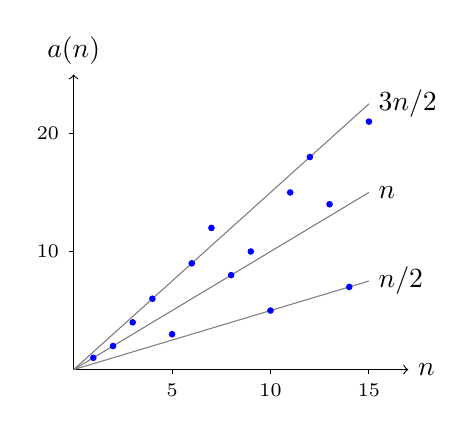
\begin{tikzpicture}[x=0.25cm,y=0.15cm]
\draw[->] (0,0) -- (17,0) node[right] {$n$};
\draw[->] (0,0) -- (0,25) node[above] {$a(n)$};
\foreach \x in {5,10,15} \draw (\x,0) -- (\x,-0.35) node[below] {\scriptsize \x};
\foreach \y in {10,20} \draw (0,\y) -- (-0.25,\y) node[left] {\scriptsize \y};
\draw[gray] (0,0) -- (15,7.5) node[right,black] {$n/2$};
\draw[gray] (0,0) -- (15,15) node[right,black] {$n$};
\draw[gray] (0,0) -- (15,22.5) node[right,black] {$3n/2$};
\foreach \x/\y in {1/1,2/2,3/4,4/6,5/3,6/9,7/12,8/8,9/10,10/5,11/15,12/18,13/14,14/7,15/21}
  \fill[blue] (\x,\y) circle (1.2pt);
\end{tikzpicture}
\caption{The first fifteen terms and the three critical lines.}\label{fig:branches}
\end{figure}

\subsection*{The diagonal, three lines and cycles}\label{sec:consequences}
The second-order term settles these diagonal questions.

Thomas Ordowski conjectured ``If $a(n)\neq p$, then almost
everywhere $a(n)>n$'' and ``$\lim\#(a_n>n)/n=1$''
\cite[A064413, comments, January 23, 2009]{oeis}. Artur Jasinski conjectured finiteness of A152458 ($a(k)=k$) and
A152519
\cite[A152458 and A152519, comments, December 2008]{oeis}.
Here $p$ denotes a prime.

Hofman--Pilipczuk \cite[Theorem~4.17]{hp} and Haver
\cite[Corollary~12(c)]{haver} establish $b(n)/n\to1$.
Our counting argument below already gives from this ratio
$\#\{k\leq N:a(k)\text{ prime}\}\sim N/(2\log N)$.
The new conclusion $b(n)>n$ for all large $n$ identifies these prime-value
indices, up to finitely many exceptions, with those below the diagonal.

\begin{lemma}\label{lem:window}
For every $\eta>0$ there is $N_0\geq3$ such that $n<b(n)\leq(1+\eta)n$
for all $n\geq N_0$. For every $n$, exactly one of the following holds:
$a(n)$ is an odd prime and $b(n)=2a(n)$; $a(n)=3p$ for an odd prime $p$
and $2a(n)=3b(n)$; or $b(n)=a(n)$.
\end{lemma}
\noindent The elementary inequalities are verified in Appendix~\ref{detail-lemma-window}.


\begin{corollary}[The diagonal]\label{cor:sign}
For all sufficiently large $n$, $a(n)<n$ if $a(n)$ is prime and
$a(n)>n$ if $a(n)$ is not prime. Thus, apart from finitely many $n$,
$a(n)>n$ exactly when $a(n)$ is composite, and $a(n)\neq n$. Moreover,
as $N\to\infty$,
\[
 \#\{k\leq N:a(k)<k\}\sim\frac{N}{2\log N},\qquad
 \#\{k\leq N:a(k)>k\}=N-\Bigl(\frac12+o(1)\Bigr)\frac{N}{\log N}.
\]
In particular $\#\{k\leq N:a(k)>k\}/N\to1$.
\end{corollary}
\begin{proof}
Take $N_0$ from Lemma~\ref{lem:window} with $\eta=1/3$, and let
$n\geq N_0$. If $a(n)$ is prime, it is not $2$, since $b(n)>n\geq3$;
so $a(n)=b(n)/2\leq2n/3<n$. If $a(n)$ is not prime, it is not $1$
(else $b(n)=1<n$), and either $a(n)=b(n)>n$ or $a(n)=3b(n)/2>n$.

For the counts, fix $\eta\in(0,1/3]$ and its $N_0$. For $N\geq N_0$,
the sets $\{k\leq N:a(k)<k\}$ and $\{k\leq N:a(k)\text{ prime}\}$ agree
on $[N_0,N]$, and $a(k)=k$ only for $k<N_0$. Let $P(N)$ be the number
of $k\in[N_0,N]$ with $a(k)$ prime. Each such $k$ has
$a(k)=b(k)/2\leq(1+\eta)N/2$, and $a$ is injective, so
$P(N)\leq\pi((1+\eta)N/2)$. Conversely, let
$M=\max\{a(k):k<N_0\}$. Since $a$ is a permutation, each prime $p$
with $M<p\leq N/2$ is $a(k)$ for one $k$, and $k\geq N_0$ because
$p>M$. Then $k<b(k)=2p\leq N$, so $P(N)\geq\pi(N/2)-M$. By the prime
number theorem $\pi(cN)\sim cN/\log N$ for each fixed $c>0$, hence
\[
 1-o(1)\leq\frac{P(N)}{N/(2\log N)}\leq1+\eta+o(1),
\]
and $\eta$ is arbitrary. The second count is $N$ minus the first and
minus the finitely many $k$ with $a(k)=k$.
\end{proof}

Corollary~\ref{cor:sign} strengthens Ordowski's first conjecture and proves Ordowski's second.

Corollary~\ref{cor:sign} also gives finiteness of Ordowski's A155549,
the nonprime values $a(n)<n$, and A064420, the $k$ with $a(k+1)=k$.
The short deductions are in Appendix~\ref{sec:uniform-details}.
De Vlieger \cite{devlieger} called finiteness of A064420 ``not surprising''.

\begin{corollary}[Three lines]\label{cor:lines}
Each of the sets $\{k:2a(k)=k\}$, $\{k:a(k)=k\}$ and $\{k:2a(k)=3k\}$
is finite.
\end{corollary}
\noindent The elementary inequalities are verified in Appendix~\ref{detail-corollary-lines}.


In fact the ratios $a(n)/n$ eventually lie in
$(1/2,2/3]\cup(1,4/3]\cup(3/2,2]$, avoiding $1/2$, $1$ and $3/2$.
The finiteness results do not establish completeness of the OEIS lists;
Amiram Eldar recorded in 2024 that neither A152458 nor A152519 has a
further term below $10^5$ \cite[A152458 and A152519, Eldar comments, 2024]{oeis}.

LRS write ``The experimental evidence suggests that there are infinitely many finite cycles and infinitely many
infinite cycles'' \cite[Section~7]{lrs}; we treat bounded cycle lengths:

\begin{corollary}[Short cycles]\label{cor:cycles}
For each $L\geq1$, the permutation $n\mapsto a(n)$ of the positive
integers has only finitely many cycles of length at most $L$.
\end{corollary}
In the cycle proof, $(\sigma,\tau)=(0,0),(1,0),(1,1)$ correspond to
unchanged values, odd primes and three times odd primes; $L$ bounds cycle length.

\begin{proof}
By Lemma~\ref{lem:window}, for each $n$,
\[
 2^{\sigma(n)}a(n)=3^{\tau(n)}b(n),\qquad
 (\sigma(n),\tau(n))\in\{(0,0),(1,0),(1,1)\}.
\]
Choose $\eta>0$ with
$(1+\eta)^L<2^L/(2^L-1)$, and $N_0$ for this $\eta$. Suppose a cycle
$x_1,\ldots,x_\ell$, with $a(x_i)=x_{i+1}$ for $i<\ell$,
$a(x_\ell)=x_1$ and $\ell\leq L$, has every $x_i\geq N_0$. Since $a$ permutes the $x_i$,
$\prod a(x_i)=\prod x_i$; with $u=\sum\sigma(x_i)$ and
$v=\sum\tau(x_i)$, so $v\leq u\leq\ell$,
\[
 2^u\prod_{i=1}^{\ell}x_i=3^v\prod_{i=1}^{\ell}b(x_i).
\]
As $b(x_i)>x_i$, this forces $3^v<2^u$, so $u\geq1$ and
$3^v\leq2^u-1$. As $b(x_i)\leq(1+\eta)x_i$, the right side is then at
most $(2^u-1)(1+\eta)^{\ell}\prod x_i$, which is less than
$2^u\prod x_i$ because
$(1+\eta)^\ell<2^L/(2^L-1)\leq2^u/(2^u-1)$. This contradiction shows
that every cycle of length at most $L$ contains an integer below
$N_0$. Distinct cycles are disjoint, so there are fewer than $N_0$ of them.
\end{proof}

\section{Formal verification}\label{sec:lean}
The formal statement matches Theorem~\ref{thm:main}:
Theorem \texttt{ekg\_sharp\_all\_index} states that every
real $\eps>0$ admits a natural $N\geq3$ for which all natural
$n\geq N$ satisfy
\[
 \left|b(n)-n-\frac{n}{3\log n}\right|
       \leq \eps\frac{n}{\log n}.
\]
The canonical sequence follows \eqref{eq:rule}: it starts $1,2$ and then chooses the
least unused positive integer not coprime to its predecessor.
The paper uses positive indices; the formal sequence extends to zero
by $a(0)=1$.
Smoothing \eqref{eq:smooth} fixes $2,6$. Arithmetic is real, logarithms natural, and there are no additional
hypotheses. The proof uses propositional extensionality,
classical choice and quotient soundness. Unproved library
declarations lie outside its dependencies.
We use Lean \cite{lean}, mathlib \cite{mathlib} and the prime
number theorem library \cite{pntcode}. Our Lean proof imports Haver's formal proofs of the estimates
(Proposition~\ref{prop:inputs}) and checks their weakenings from the
canonical definition. The formal proof derives the asymptotic directly
from these estimates and counting identities. Haver's upper bound and
criterion enter only the comparison with Haver's results.

Haver's Lean archive already proves the general counting identities
\cite[Corollary~12(b)]{haver};
our proof discharges their prime-interval and tick endpoint hypotheses
and derives the coefficient and all-index transfer. Haver's sharp upper bound and second-order
criterion lie outside Haver's archive's verified core
\cite[verification note, ``Claims outside the checked coverage'']{haver}. Lean also checks the sign, density, below-diagonal count, three-line and
exceptional-set finiteness, and bounded-cycle finiteness; the three-branch
formulas (Corollary~\ref{cor:branches}) and the second count in
Corollary~\ref{cor:sign} are deductions outside Lean.

\paragraph{Acknowledgments.}
The author thanks Tomer Haver for the estimates, counting identity,
reduction and accompanying Lean sources.

\clearpage
\begin{appendices}
\section{Routine estimates}\label{sec:uniform-details}
We record the uniform parameter choices and the elementary inequalities
used in the consequences.

\paragraph{Constants in the established estimates.}
The constants $793=12\cdot6+721$ and $802=13\cdot6+724$ are convenient
weakenings using $\pi(\sqrt e)\leq6\sqrt e/\log e$ and
$\sqrt e/\log e\geq1$ eventually; $C_1=4\cdot793^2+2\cdot793$ suffices.

\paragraph{Parameters for Proposition~\ref{prop:upper}.}\label{detail-uniform-2}
The constants $A$ and $\eta$ in the interval and sieve bounds may be chosen
as follows.
% EKG proof fragment 9485dce2a6d1248c-1 begin
All constants in this proof are chosen before the
final threshold on $t$. % EKG proof fragment 9485dce2a6d1248c-1 end
% EKG proof fragment 9485dce2a6d1248c-3 begin
For example, $A=C_1+8C+1$ suffices.
% EKG proof fragment 9485dce2a6d1248c-3 end
% EKG proof fragment 9485dce2a6d1248c-5 begin
Choose $\eta=\delta/(32AM)$ after fixing $M$. % EKG proof fragment 9485dce2a6d1248c-5 end
% EKG proof fragment 9485dce2a6d1248c-7 begin
The frontier tends to infinity, so one threshold
on $t$ works for every later prefix. This proves the proposition.% EKG proof fragment 9485dce2a6d1248c-7 end

\paragraph{Parameters for Proposition~\ref{prop:lower}.}\label{detail-uniform-3}
Here $s$ is the fixed factor of the missing composite, and $u$ is a
selected successor; the factorization $u=sq_y$ uses that fixed factor.
% EKG proof fragment 245802c9ff78e4ac-1 begin
This does not assert that
$s=\spf(u)$.% EKG proof fragment 245802c9ff78e4ac-1 end

% EKG proof fragment 245802c9ff78e4ac-3 begin
Fix $\eta=\delta/(16MA_B)$. % EKG proof fragment 245802c9ff78e4ac-3 end
% EKG proof fragment 245802c9ff78e4ac-5 begin
The choices have the order $\delta$, the upper-excursion cutoff,
$M$, $\eta$, $C_\eta$, and finally the frontier and index cutoffs.
All are uniform in the missing composite $h$ and the selected $y$.% EKG proof fragment 245802c9ff78e4ac-5 end

\paragraph{Quantifiers for Theorem~\ref{thm:main}.}\label{detail-quantifiers}
In the following verification, the clock estimates are \eqref{eq:clock},
the excursion propositions are Propositions~\ref{prop:upper}--\ref{prop:lower},
and finite seed exclusions mean the finitely many initial indices omitted
by their eventual estimates. The upper-excursion cutoff above is the
threshold in Proposition~\ref{prop:upper}.
% EKG proof fragment 5f145292b58f1021-1 begin
For completeness, the uniform little-$o$ conclusions here give exactly
the quantifiers in \eqref{eq:epsilon}. Given $\eps>0$, apply the two
excursion propositions with $\delta=\eps/8$. Eventually
$L(E(n-1))\leq2L(n)$, so their contribution is at most
$\eps L(n)/4$. Take a common cutoff for the clock estimates shifted
by $1,2,3$, each with error at most $\eps L(n)/2$, and for the
finite seed exclusions. Their sum is at most $\eps L(n)$ at every
ordinary index; the shifted clock alone covers the prime blocks.
Increasing the common cutoff to at least $3$ proves the theorem.% EKG proof fragment 5f145292b58f1021-1 end

\label{detail-lemma-window}
\begin{proof}[Proof of Lemma~\ref{lem:window}]
Apply \eqref{eq:epsilon} with $\eps=1/6$: for $n\geq N$,
$b(n)\geq n+n/(6\log n)>n$ and $b(n)\leq n+n/(2\log n)$, which is at
most $(1+\eta)n$ once $\log n\geq1/(2\eta)$. The second statement is
the definition \eqref{eq:smooth}.
\end{proof}

\label{detail-corollary-lines}
\begin{proof}[Proof of Corollary~\ref{cor:lines}]
Take $N_0$ from Lemma~\ref{lem:window} with $\eta=1/3$, and let
$n\geq N_0$, so $n<b(n)\leq4n/3$. If $a(n)$ is an odd prime, then
$2a(n)=b(n)$, so $n<2a(n)\leq4n/3$. If $a(n)=3p$ for an odd prime $p$,
then $2a(n)=3b(n)>3n$. Otherwise $a(n)=b(n)$ and $2n<2a(n)\leq8n/3$.
In no case is $2a(n)$ equal to $n$, $2n$ or $3n$, so all three sets
lie in $[1,N_0)$.
\end{proof}

\paragraph{The exceptional OEIS sets.}
By Corollary~\ref{cor:sign} the indices
$n$ with $a(n)$ not prime and $a(n)\leq n-1$ form a finite set, so its
image A155549 is finite. For the
second, $a(n)=n-1$ fails for large $n$: a prime value has
$a(n)\leq2n/3$ and any other value has $a(n)>n$.

\section{Numerical illustration}\label{sec:numerics}
Table~\ref{tab:ratio} displays $R(n)=(b(n)-n)\log n/n$, computed by the
recursive greedy rule \eqref{eq:rule} with prime-factor sieving.
\begin{table}[ht]
\centering
\begin{tabular}{r r r}
$n$ & $b(n)$ & $R(n)$\\\hline
1,000 & 1,043 & 0.2970 \\
10,000 & 10,361 & 0.3325 \\
100,000 & 103,088 & 0.3555 \\
1,000,000 & 1,024,686 & 0.3410 \\
10,000,000 & 10,210,804 & 0.3398 \\
100,000,000 & 101,839,957 & 0.3389 \\
500,000,000 & 508,457,544 & 0.3388 \\
\end{tabular}
\caption{The normalized smoothed error, rounded to four decimal places; Theorem~\ref{thm:main} gives its limit $1/3$.}\label{tab:ratio}
\end{table}

\paragraph{Related work.}
Haver's Yellowstone papers \cite{haverY3,haverYFrontier,haverY6,haverY7,haverY8} are unused.

\end{appendices}
\clearpage
Other nearby visiting rules include Applegate, Havermann, Selcoe,
Shevelev, Sloane and Zumkeller's Yellowstone permutation~\cite{yellowstoneOriginal},
Basistha and Iona\c{s}cu's coprime permutation~\cite{basisthaIonascu}, and
Na's real-multiplier process~\cite{naVisiting}. Nothing from these works is used here.

\begin{thebibliography}{99}

\bibitem{haverY3}
T. Haver, \emph{The Yellowstone permutation, III: few large terms}, October 22, 2026.
\href{https://doi.org/10.5281/zenodo.23557280}{doi:10.5281/zenodo.23557280}.

\bibitem{haverYFrontier}
T. Haver, \emph{The prime frontier of the Yellowstone permutation is linear}, October 22, 2026.
\href{https://doi.org/10.5281/zenodo.23558450}{doi:10.5281/zenodo.23558450}.

\bibitem{haverY6}
T. Haver, \emph{The prime frontier of the Yellowstone permutation falls behind time: limsup R(t)/t < 1}, October 23, 2026.
\href{https://doi.org/10.5281/zenodo.23604646}{doi:10.5281/zenodo.23604646}.

\bibitem{haverY7}
T. Haver, \emph{The Yellowstone permutation: limsup R(t)/t $\leq$ 0.68605, liminf n\_p/p $>$ 1.4576, and Conjecture 7 for large n}, October 23, 2026.
\href{https://doi.org/10.5281/zenodo.23604811}{doi:10.5281/zenodo.23604811}.

\bibitem{haverY8}
T. Haver, \emph{The Yellowstone permutation: Conjecture 7 for all n reduced to a riser law on a finite range, the normality and entry times of primes, and a run certificate}, October 23, 2026.
\href{https://doi.org/10.5281/zenodo.23604970}{doi:10.5281/zenodo.23604970}.


\bibitem{sievebook}
A. C. Cojocaru and M. R. Murty, \emph{An Introduction to Sieve Methods
and Their Applications}, LMS Student Texts \textbf{66}, Cambridge
University Press, 2005, Sections 5.1--5.2.
\href{https://doi.org/10.1017/CBO9780511615993}{doi:10.1017/CBO9780511615993}.

\bibitem{lean}
L. de Moura and S. Ullrich, The Lean 4 theorem prover and programming
language, in \emph{Automated Deduction---CADE 28}, LNCS \textbf{12699},
Springer, 2021, pp. 625--635.
\href{https://doi.org/10.1007/978-3-030-79876-5_37}{doi:10.1007/978-3-030-79876-5\_37}.

\bibitem{poussin}
Ch.-J. de la Vall\'ee Poussin, Recherches analytiques sur la th\'eorie
des nombres premiers. Premi\`ere partie: Les nombres premiers en g\'en\'eral,
\emph{Ann. Soc. Sci. Bruxelles} \textbf{20}, deuxi\`eme partie (1896),
Section~56 (\emph{Digitized collected offprint}, 1897, pp.~67--69).
\href{https://archive.org/details/recherchesanaly00pousgoog}{Original offprint}.

\bibitem{devlieger}
M. De Vlieger, Constitutive analysis of the EKG sequence, 2021,
\url{https://vincico.com/seq/a064413.html}.

\bibitem{ekgbounds}
P. Graham, Sharp linear bounds for the EKG sequence, version 1,
October 22, 2026, manuscript and Lean sources.
\href{https://doi.org/10.5281/zenodo.23562177}{doi:10.5281/zenodo.23562177}.

\bibitem{hadamard}
J. Hadamard, Sur la distribution des z\'eros de la fonction $\zeta(s)$
et ses cons\'equences arithm\'etiques,
\emph{Bull. Soc. Math. France} \textbf{24} (1896), 199--220.
\href{https://doi.org/10.24033/bsmf.545}{doi:10.24033/bsmf.545}.

\bibitem{haver}
T. Haver, Explicit rates for the EKG sequence, version 3,
October 4, 2026, manuscript and Lean sources.
\href{https://doi.org/10.5281/zenodo.23129632}{doi:10.5281/zenodo.23129632}.

\bibitem{hp}
P. Hofman and M. Pilipczuk, A few new facts about the EKG sequence,
\emph{J. Integer Sequences} \textbf{11} (2008),
\href{https://cs.uwaterloo.ca/journals/JIS/VOL11/Hofman/hofman1.html}{Article 08.4.2}.

\bibitem{pntcode}
A. Kontorovich, T. Tao, et al.,
\emph{PrimeNumberTheoremAnd} (Prime Number Theorem and More),
Lean sources, revision
\texttt{c39a751132c88b6e8080b74c74023fd95b3d8be0}, 2026.
\url{https://github.com/AlexKontorovich/PrimeNumberTheoremAnd}.

\bibitem{lrs}
J. C. Lagarias, E. M. Rains, and N. J. A. Sloane,
The EKG sequence, \emph{Experimental Math.} \textbf{11} (2002), 437--446.
\href{https://doi.org/10.1080/10586458.2002.10504486}{doi:10.1080/10586458.2002.10504486};
\href{https://arxiv.org/abs/math/0204011v1}{arXiv:math/0204011v1}.

\bibitem{mathlib}
The mathlib Community, The Lean mathematical library, in
\emph{Proceedings of CPP '20}, ACM, 2020, pp. 367--381.
\href{https://doi.org/10.1145/3372885.3373824}{doi:10.1145/3372885.3373824};
\href{https://arxiv.org/abs/1910.09336}{arXiv:1910.09336}.

\bibitem{oeis}
OEIS Foundation Inc., \emph{The On-Line Encyclopedia of Integer Sequences},
entries \href{https://oeis.org/A064413}{A064413},
\href{https://oeis.org/A064420}{A064420},
\href{https://oeis.org/A152458}{A152458},
\href{https://oeis.org/A152519}{A152519},
\href{https://oeis.org/A155549}{A155549} and
\href{https://oeis.org/A256417}{A256417}.


\bibitem{yellowstoneOriginal}
David L. Applegate, Hans Havermann, Robert G. Selcoe, Vladimir Shevelev,
N. J. A. Sloane and Reinhard Zumkeller,
\emph{The Yellowstone Permutation},
arXiv:1501.01669, first posted January 7, 2015; version~2, March 8, 2015.
\url{https://arxiv.org/abs/1501.01669v2}.

\bibitem{basisthaIonascu}
Amit Kumar Basistha and Eugen J. Iona\c{s}cu,
\emph{A special sequence and primorial numbers},
arXiv:2302.02838, first posted February 6, 2023; version~5, November 22, 2023.
Rev. Roumaine Math. Pures Appl. 70 (2025), 235--255.
\url{https://arxiv.org/abs/2302.02838v5}.
\url{https://doi.org/10.59277/rrmpa.2025.235.255}.

\bibitem{naVisiting}
Sungsoo Na,
\emph{An integer-visiting process with real multipliers: coverage and rates},
version~1.0.0, October 4, 2026.
\url{https://doi.org/10.5281/zenodo.23138274}.

\end{thebibliography}

\bigskip
\noindent 2020 \emph{Mathematics Subject Classification}:
Primary 11B83; Secondary 11A05, 68V15.\\
\emph{Keywords}: EKG sequence, greedy permutation, prime number theorem,
asymptotic formula, formal verification.\\
\emph{Concerned with sequences}
\href{https://oeis.org/A064413}{A064413},
\href{https://oeis.org/A064420}{A064420},
\href{https://oeis.org/A155549}{A155549},
\href{https://oeis.org/A152458}{A152458},
\href{https://oeis.org/A152519}{A152519} and
\href{https://oeis.org/A256417}{A256417}.

\end{document}
